%\documentclass[12pt,a4paper]{report}
\documentclass[12pt,a4paper,oneside,onecolumn,openright]{book}
% set the document language
\usepackage[italian]{babel}
% set the encoding used by your editor here (default is utf8)
\usepackage[utf8]{inputenc}
\usepackage[T1]{fontenc}

% math packages
\usepackage{amsmath}
\usepackage{amssymb}
\usepackage{lmodern}
% page margins settings
\usepackage[inner=3cm,outer=2.5cm,top=3cm,bottom=2.5cm]{geometry}
%\usepackage{indentfirst}

% other packages
\usepackage{array}
\usepackage{enumitem}
\usepackage{subfigure}
\usepackage{graphicx}
\usepackage{verbatim}
\usepackage{listings}
\usepackage{url}
\usepackage[hidelinks]{hyperref}
\usepackage[export]{adjustbox}
\usepackage{latexsym}
\usepackage{tabularx}
\usepackage{ragged2e}
\usepackage{mathtools}
\DeclarePairedDelimiter\floor{\lfloor}{\rfloor}
\DeclarePairedDelimiter\ceil{\lceil}{\rceil}
% \usepackage{Mathematics}
% custom colors
\usepackage{color}
\usepackage{wrapfig}
\usepackage{gensymb}
\usepackage{caption}
\usepackage{tikz}
\usepackage{forest}
\usepackage{tikz-qtree}
\usetikzlibrary{positioning, shapes.geometric}
\usetikzlibrary{shapes.geometric, arrows.meta, positioning, fit}
\tikzstyle{block} = [thick, text width=.4cm, minimum height=.5cm, align=center]  


\usetikzlibrary{shadows}
\definecolor{light-gray}{gray}{0.96}
\definecolor{cyan}{RGB}{230,230,255}
\definecolor{dkgreen}{rgb}{0,0.6,0}
\definecolor{gray}{rgb}{0.5,0.5,0.5}
\definecolor{mauve}{rgb}{0.58,0,0.82}
\definecolor{iceberg}{rgb}{0.44, 0.65, 0.82}
% \definecolor{blue}{RGB}{44, 44, 210}

\hypersetup{
colorlinks=true,
linkcolor=black,
% filecolor=blue,
urlcolor=blue,
% pdftitle={Overleaf Example},
}

\urlstyle{same}
\graphicspath{ {./images/} }

% environment for bash code
\lstset{ %
  language=bash,                % the language of the code
  basicstyle=\footnotesize,           % the size of the fonts that are used for the code
  numbers=left,                   % where to put the line-numbers
  numberstyle=\footnotesize,          % the size of the fonts that are used for the line-numbers
  stepnumber=1,                   % the step between two line-numbers. If it's 1, each line 
                                  % will be numbered
  numbersep=5pt,                  % how far the line-numbers are from the code
  backgroundcolor=\color{white},      % choose the background color. You must add \usepackage{color}
  showspaces=false,               % show spaces adding particular underscores
  showstringspaces=false,         % underline spaces within strings
  showtabs=false,                 % show tabs within strings adding particular underscores
%  frame=single,                   % adds a frame around the code
  rulecolor=\color{black},        % if not set, the frame-color may be changed on line-breaks within not-black text (e.g. commens (green here))
  tabsize=2,                      % sets default tabsize to 2 spaces
  captionpos=b,                   % sets the caption-position to bottom
  breaklines=true,                % sets automatic line breaking
  breakatwhitespace=false,        % sets if automatic breaks should only happen at whitespace
  title=\lstname,                   % show the filename of files included with \lstinputlisting;
                                  % also try caption instead of title
  numberstyle=\tiny\color{gray},        % line number style
  keywordstyle=\textbf,          % keyword style
  commentstyle=\color{dkgreen},       % comment style
%  stringstyle=\color{mauve},         % string literal style
  escapeinside={\%*}{*)},            % if you want to add a comment within your code
  morekeywords={*,...,insert,-}               % if you want to add more keywords to the setù
}

% environment for python code
\lstset{
	language=Python,
	breaklines=true,
	breakatwhitespace=true ,
	backgroundcolor=\color{light-gray}
}

\newcommand{\grayScale}{0.95} % Can change the gray level here
\definecolor{codeBackground}{rgb}{\grayScale ,\grayScale ,\grayScale}
\definecolor{forestGreen}{rgb}{0.13,0.55,0.13}

\lstset{
    language=C,
    backgroundcolor=\color{codeBackground},
    tabsize=4,
    showstringspaces=false,
    showtabs=false,
    showspaces=false,
    basicstyle=\ttfamily,
    identifierstyle=\ttfamily,
    keywordstyle=\color{blue},
    stringstyle=\color{red},
    commentstyle=\color{gray},
    numberstyle=\color{magenta},
    morecomment=[l][\color{forestGreen}]{\#},
    escapechar={|}, 
}
% appendices package
%\usepackage{appendix}
% set Appendix name used in the toc
%\renewcommand{\appendixtocname}{Appendice}

% interline
\linespread{1.5}
% set numbers for subsections and show them in the toc
\setcounter{tocdepth}{3} 
\setcounter{secnumdepth}{3}

% layout package, style and settings
\usepackage{fancyhdr}
\pagestyle{fancy}

\fancypagestyle{mainmatter}{%		
		\fancyhf{} 
		\fancyhead{}
		\fancyhead[LE,RO]{\thepage}
		\fancyhead[LO]{\footnotesize{\leftmark}}
		\fancyhead[RE]{\footnotesize{\rightmark}}
		\fancyfoot{}
		\addtolength{\headwidth}{\marginparsep}
		\addtolength{\headheight}{2.5pt}
		\renewcommand{\headrulewidth}{0.3pt}
		\renewcommand{\footrulewidth}{0.0pt}
		}
\fancypagestyle{frontmatter}{%
		\fancyhf{} 
		\fancyhead[LE]{\footnotesize{\MakeUppercase{\thepage}}}
		\fancyhead[RO]{\footnotesize{\MakeUppercase{\thepage}}}
		\fancyhead[RE,LO]{}
		\fancyfoot{}
		\addtolength{\headwidth}{\marginparsep}
		\addtolength{\headheight}{2.5pt}
		\renewcommand{\headrulewidth}{0.0pt}
		\renewcommand{\footrulewidth}{0.0pt}
		}
		
		
\usepackage{fancyhdr}
\pagestyle{fancy}
		\fancyhf{} 
		\fancyhead{}
		\fancyhead[LE,RO]{\thepage} 
		\fancyhead[LO]{\footnotesize{\leftmark}}
		\fancyhead[RE]{\footnotesize{\rightmark}}
		\fancyfoot{}
		\addtolength{\headwidth}{\marginparsep}
		\addtolength{\headheight}{2.5pt}
		\renewcommand{\headrulewidth}{0.3pt}
		\renewcommand{\footrulewidth}{0.0pt}

% empty pages have no numbers
\makeatletter
\def\cleardoublepage{\clearpage\if@twoside \ifodd\c@page\else
\hbox{}
  %Potresti voler togliere il commento dalla linea seguente
  %Questa pagina � stata lasciata intenzionalmente vuota.
\thispagestyle{empty}
\newpage
\if@twocolumn\hbox{}\newpage\fi\fi\fi}
\makeatother
%????
%\textwidth=450pt\oddsidemargin=0pt

%\makeatletter 
%  \DeclareRobustCommand*\textsubscript[1]{% 
%    \@textsubscript{\selectfont#1}} 
%  \newcommand{\@textsubscript}[1]{% 
%    {\m@th\ensuremath{_{\mbox{\fontsize\sf@size\z@#1}}}}} 
\makeatother 

\begin{document}
\begin{titlepage}
\begin{center}
{
    \large
    \textbf{Università  degli studi di Modena e Reggio Emilia} \\
   	\textbf{Dipartimento di Ingegneria Enzo Ferrari} \\
    \vspace{\stretch{0.5}}
    \hspace*{0cm} \hrulefill \hspace*{0cm} \\
    \vspace{\stretch{0.5}}    
	  \vspace{\stretch{12}}
  
  
 		\huge{\bf Real Time Embedded System }}\\
		\vspace{3mm}
		
		\vspace{\stretch{6}}
		\end{center}
		
\vspace{40mm}
\par
\noindent
\vspace{20mm}
\begin{center}
\hspace*{0cm} \hrulefill \hspace*{0cm} \\
{\large{\bf 
Anno Accademico 2023/24}}
\end{center}

\end{titlepage}

\pagestyle{frontmatter}
\frontmatter

% PAGINA VUOTA
%\clearpage\null\thispagestyle{empty}\clearpage
\setcounter{tocdepth}{2}
\tableofcontents

\setlength{\parindent}{12pt}
\setlength{\parskip}{1ex plus 0.5ex minus 0.2ex}
\mainmatter
\pagestyle{mainmatter}

\chapter{Introduction}

\section{Structure and Content}
\begin{itemize}

    \item \textbf{Module 1}: 
    \begin{enumerate}
        \item \textbf{\textit{intra-vehicles communications}}: nodes, sensors, ECU
        \item \textbf{\textit{signal busses}}: CAN, LIN, FlexRay, MOST, Ethernet [ T1/T1S]
        \item \textbf{\textit{car domain and OS}}
    \end{enumerate}
    
    \item \textbf{Module 2}:
    \begin{enumerate}
        \item \textbf{\textit{inter-vehicles communications}}: \textit{V2V} and \textit{V2X} (car is a node)
        \item \textbf{\textit{wireless technologies}}: Bluetooth, LoRa, C-V2X, IEE 802.11p (bd)
        \item application, messages, broadcast, GPS
    \end{enumerate}

\end{itemize}
Different \textbf{domain} or \textbf{application} needs different \textit{communications protocols}, is important to understand how each nodes in domain communicate each other (inside the car).

\newpage
\section{Intra-Vehicles}
From the 80's, where the car's control unit are isolated an there was a dedicated wires connect sensors and actuators with less electronic than now, until the reach the greates goal of evolution in the automotive sector: autonomous drive. The complexity of the number of connection from each ECU's to the other, also the number of ECU's for each car, is growing. While the number of signal increase in a liner way, the connection between ECU's is growing with a quadratic complexity $O(n^2)$.

If we examine the evolutions of the ECUs number inside an ``Audi A6'' we can observe that in 1997 it has 5 ECUs and in the 2007 it has 50 ECUs, instead the ``Tesla M3'' in the 2017 has 70 ECUs. The quadratic increase of ECUs number, however has reach a cap for two main reason: the cost and the space inside the car. Traditionally one ECUs is responsible of one task, but nowadays it could be two type of trends:
\begin{enumerate}[nosep]
    \item \textit{distributed of function across ECUs}
    \item \textit{integration of multiple function in one ECU}
\end{enumerate}

\section{Architectures}

\begin{figure}[h]
    \centering
    \begin{minipage}[t]{0.45\textwidth}
        \centering
        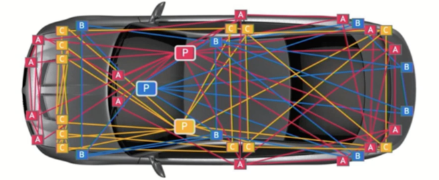
\includegraphics[width=\textwidth]{img/domain_architecture}
        \caption{\textit{Domain Architecture}}
        
        \begin{flushleft}
            \begin{enumerate}[nosep]
                \item central domain controller (\textbf{P}) or high performance computer
                \item ability to handle more complex functions
                \item cost optimization
                \item cable harness is rigid and expensive
            \end{enumerate}
        \end{flushleft}

    \end{minipage}
    \begin{minipage}[t]{0.45\textwidth}
        \centering
        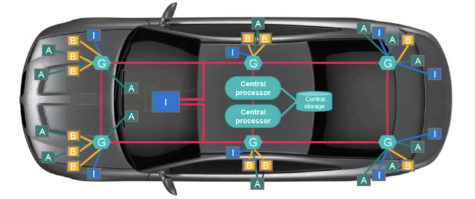
\includegraphics[width=\textwidth]{img/zonal_architecture}
        \caption{\textit{Zonal Architecture}}
        
        \begin{flushleft}
            \begin{enumerate}[nosep]
                \item local ethernet per zone (\textbf{G})
                \item ultra high-speed secured backbone between zone
                \item centralized software
                \item central computer storage
            \end{enumerate}
        \end{flushleft}
        
    \end{minipage}
\end{figure}
\chapter{Non Real-time scheduling algorithms}
Lo \textit{scheduling} è l'attività che permette di selezionare quale processo o \textit{thread} bisogna eseguire come successivo. In generale nei sistemi operativi, possiamo distinguere tre tipologie di \textit{scheduling}:
\begin{itemize}
    \item \textbf{\textit{long term scheduling}}: prima di creare il processo, viene deciso se attivarlo o meno. Viene implementato tramite un \textbf{test di ammissione}, se il processo passa questo controllo allora viene inserito nella \textit{ready queue}, se no viene interrotto finché non gli viene permesso di essere \textit{schedulato} [ se il \textit{load} del processore è troppo alto il nuovo task rischia di essere solo di ``intralcio'' ].
    \item \textbf{\textit{medium term scheduling}}: permette di decidere se un processo deve essere \textit{preemptato} o meno.
    \item \textbf{\textit{short term scheduling}}: decide quale processo deve essere eseguito come successivo. Possiamo distinguere:
    \begin{itemize}
        \item \textbf{\textit{selection function}}: decide quale processo viene selezionato dalla \textit{ready queue}, seguendo alcune regole.
        \item \textbf{\textit{decision mode}}: quando la decisione è stata presa si può comportare in maniera \textbf{\textit{preemptive}} oppure \textbf{\textit{non-preemptive}}.
    \end{itemize}
\end{itemize}
\textbf{\textit{Scheduling Criteria}}: come si possono valutare le performance di uno \textit{scheduler}:
\begin{itemize}
    \item \textbf{\textit{user-oriented}}: si va ad analizzare il \textit{response-time} del processo.
    \item \textbf{\textit{system-oriented}}: si va ad analizzare il \textit{throughput}, ovvero quanto lavoro il sistema può eseguire in un certo intervallo di tempo.
\end{itemize}
Per quanto le performance siano importanti in certe circostate ci possono interessare la \textbf{predicibitilà} (\textit{real-time system}) o la \textbf{\textit{fairness}}. \\
Tra i processi possiamo differenziare anche il tipo di risorsa che viene utilizzanta: \textbf{\textit{CPU-Bound}} e \textbf{\textit{I/O Bound}}, nel primo caso il processo è orientato a lavorare sul processore, mentre nel secondo caso i processi possono essere in attesa di un \textit{I/O device}. La stragrande maggioranza dei processi è un mix dei due. \\ \newline
Uno \textit{schedule} $\sigma$ si dice \textbf{fattibile} (\textbf{\textit{feasible}}) se tutti i \textit{tasks} sono capaci di completare entro un insieme di vincoli. \\
Un \textit{tasks set} $\mathcal{T}$ si dice \textbf{\textit{schedulable}} se esiste uno \textit{schedule} fattibile per esso. \\ \newline
\textbf{\textit{The General Scheduling Problem}}: dato un \textit{tasks set} $\mathcal{T}$ di $n$ \textit{tasks}, un set $\mathcal{P}$ di $m$ processori e un set $\mathcal{R}$ di $r$ risorse, trovare un assegnamento di $\mathcal{P}$ e $\mathcal{R}$ per $\mathcal{T}$ che produce uno \textit{schedule} fattibile. \\
È stato dimostrato nel 1975 da Garey e Johnson che il \textit{general scheduling problem} rientra nella categoria \textbf{\textit{NP hard}}. È però possibile, rilassando i vincoli e specificando certe condizioni, ricordurci ad un algoritmo \textit{polynomial time}. \\
Per il ora consideriamo:
\begin{itemize}
    \item processore singolo
    \item \textit{fully preemptive tasks}
    \item attivazione simultanea
    \item nessun vincolo di precedenza
    \item nessun vincolo sulle risorse
\end{itemize}

\begin{tabular}{ |p{7.25cm}|p{7.25cm}| }
    \hline
    \multicolumn{2}{|c|}{\textbf{Algorithm taxonomy}} \\
    \hline
    \textbf{\textit{preemptive}} & \textbf{\textit{non-preemptive}} \\
    \hline
    \textbf{\textit{off line}}: & \textbf{\textit{on line}}: \\
    tutte le decisioni sullo scheduling vengono prese prima dell'attivazione dei task, normalmente lo \textit{schedule} viene salvato in una tabella (\textbf{\textit{table-driven scheduling}}) & le decisioni di scheduling vengono prese \textit{runtime} sul set dei tasks attivi \\ \hline
    \textbf{\textit{static}}: & \textbf{\textit{dynamic}}: \\
    le decisioni di scheduling vengono prese basandosi su parametri fissati, staticamente assegnati al task prima dell'attivazione & le decisioni di scheduling vengono prese su parametri che possono variare nel tempo \\ \hline
    \textbf{\textit{best effort}}: & \textbf{\textit{optimal}}: \\
    trova sempre uno \textit{schedule} fattibile, se \textbf{esiste} & fa del suo meglio per trovare uno \textit{schedule} fattibile, se esiste, ma non lo garantisce. \\ \hline
\end{tabular}
\\ \newline
Le \textit{policies} classiche di \textbf{\textit{scheduling}}, che però non sono adatte per sistemi \textit{real-time}, sono:
\begin{enumerate}

    \item \textbf{\textit{First Come First Served} (FCFS)}: assegna l'utilizzo della CPU al task basandosi sull'ordine di arrivo, non è \textit{preemptive}, è dinamico, online e \textit{best effort}. \\
    $\rightarrow$ molto \textbf{impredicibile}: il \textit{response time} è fortemente dipendente dall'ordine di arrivo dei task.

    \item \textbf{\textit{Shorter Job First} (SJF)}: seleziona il task che ha il minor \textit{computational time}, può essere sia \textit{preemptive} che \textit{non-preemptive}, è statico (il parametro $C_i$ è fissato da configurazione), può essere usato sia \textit{online} che \textit{off-line} e permette di minimizzare la \textit{response time} \textbf{media}. \\
    \textcolor{green}{\textbf{Dimostrazione dell'ottimalità di SJF}}: consideriamo uno scheduler $\sigma \neq \text{SJF}$ e un'altro scheduler $\sigma'$ che è uguale a SJF fino all'istante $f_s$
    \begin{figure}[h]
        \centering
        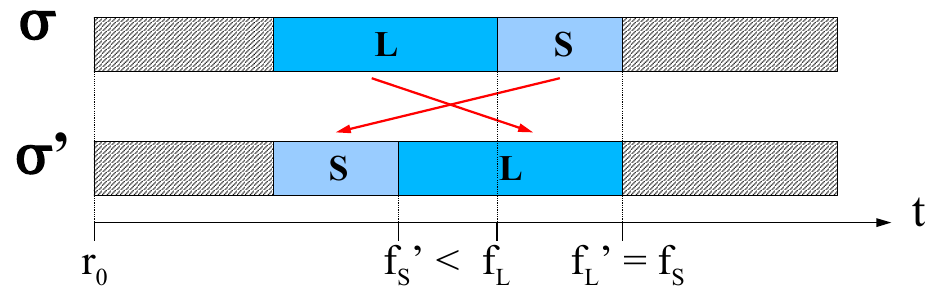
\includegraphics[width=0.4\textwidth]{img/sjf_opt}    
    \end{figure}
    \\ 
    Presi due task $L$ e $S$ che hanno \textit{request time} $r_i \; i \in \{L, S\}$ e \textit{finish time} $f_i \; i \in \{L, S\}$. Lo \textit{schedule} $\sigma$ schedula il task $L$ prima (non conforme con SJF), mentre $\sigma'$ schedula il task $S$ come primo (conforme a SJF). Possiamo dire che $f'_L = f_S$ in quanto la somma del tempo dei due task non cambia, ma cambia solo l'ordine di schedulazione. È intuitivo che il \textit{finish time} del primo task è però sbilanciato verso lo scheduler $\sigma'$ infatti avremo $f'_S < f_L$. \\
    Avremo perciò $f'_S + f'_L \leq f_S + f_L$ 
    \begin{center}
        $\rightarrow \qquad \bar{R}(\sigma') = \frac{1}{n} \cdot \sum_{i = 1}^{n}{(f'_i - r_i)} \leq \frac{1}{n} \cdot \sum_{i = 1}^{n}{(f_i - r_i)} = \bar{R}(\sigma)$
    \end{center}
    Lo scheduler $\sigma'$ è equivalente a SJF solo fino all'istante $f'_L = f_S$, bisogna andare quindi ad iterare su ogni scheduler $\sigma \in \{\sigma', \sigma'', ..., \sigma^*\}$, andando a riproporre l'analisi appena condotta avremo che: $\bar{R}(\sigma) \geq \bar{R}(\sigma') \geq \bar{R}{\sigma''} \geq \cdots \geq \bar{R}(\sigma^*)$ \\
    $\rightarrow$ $\sigma^* = \sigma_{sjf}$ e quindi avremo che $\bar{R}(\sigma_{SJF})$ è la \textbf{minima \textit{response time} media} ottenibile da ogni \textbf{algoritmo}. \\
    \textbf{SJF non è un algoritmo fattibile per il \textit{Real-Time}}.

    \item \textbf{\textit{Priority Scheduling}}
\end{enumerate}
\chapter{Real-time scheduling algorithms}
\chapter{Periodic Task Scheduling}
\textit{Scheduling} di \textit{tasks} \textbf{periodici} o \textbf{sporadici} (\textbf{aperiodici}). Definiamo un \textbf{task periodico} $\tau_i(C_i, T_i)$ con $C_i$ il \textit{worst case execution time} e $T_i$ il \textbf{periodo} per il quale il task $\tau_i$ deve essere eseguito.
\begin{figure}[h]
    \centering
    \begin{minipage}[t]{0.45\textwidth}
        \centering
        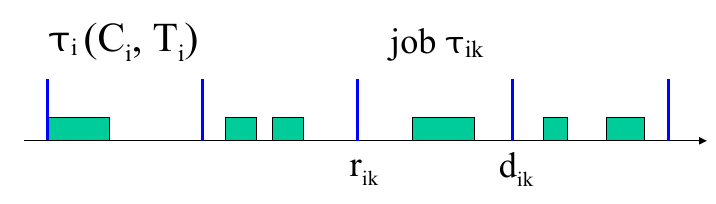
\includegraphics[width=\textwidth]{img/T_aT}
        \caption{\textit{periodic task}}
    \end{minipage}
    \begin{minipage}[t]{0.45\textwidth}
        \centering
        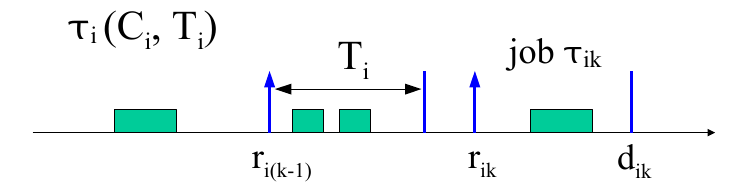
\includegraphics[width=\textwidth]{img/T_aT_1}
        \caption{\textit{sporadic task}}
    \end{minipage}
\end{figure}
\\
Per ogni task periodico, bisogna garantire che:
\begin{itemize}
    \item ogni job $\tau_{ik}$ venga attivato in $r_{ik} = (k - 1) \cdot T_i$.
    \item ogni job $\tau_{ik}$ completi la sua esecuzione entro $d_{ik} = r_{ik} + D_i$.
\end{itemize}
Anche nel caso di \textbf{task aperiodici} possiamo definirli $\tau_i(C_i,T_i)$, in questo caso però $T_i$ non è il periodo nel quale per il quale si ripete il task ma indica il \textit{deelay} minimo di attivazione tra un task $\tau_{ik}$ e un task $\tau_{i(k+1)}$, infatti bisogna garantire per ogni task sporadico che:
\begin{itemize}
    \item ogni job $\tau_{ik}$ viene attivato in un istante $r_{ik} \geq r_{i(k-1)} + T_i$.
    \item ogni job $\tau_{ik}$ completi la sua esecuzione entro una \textit{deadline} relativa $d_{ik} = r_{ik} + D_i$
\end{itemize}

\section{Timeline Scheduling}
È una tipologia di \textit{scheduling offline} è stata utilizzata per anni nei contesti in cui era richiesto un \textit{hard real time} per via della delicatezza delle circostanze di uso (sistemi militari, navigazioni e sistemi di monitoraggio). Può essere chiamato anche \textbf{\textit{cycle executive}} o \textbf{\textit{cyclic scheduling}}. \\
Il funzionamento era tale che l'asse del tempo venisse divisa in intervalli con lunghezza uguale, anche chiamati \textbf{\textit{time slots}}, ogni task viene allocato staticamente in un certo slot e in un certo ordine per venire incontro ai \textit{request rate} desiderati. L'esecuzione per ogni slot viene attivato tramite un \textbf{\textit{timer}}. Consideriamo un task set $\mathcal{T} = \{\tau_1, \tau_2, ..., \tau_k\}$ e che $\forall \tau_i \in \mathcal{T} \; \exists (C_i, T_i)$, in questo caso $T_i \equiv D_i$ ovvero che il periodo del task corrisponde con la sua \textit{deadline} assoluta. Definiremo:
\begin{itemize}
    \item il \textbf{\textit{minor cycle}} come $\Delta = gcd(T_i, T_j) \; \forall T_i, T_j \in \mathcal{T}, \; i \neq j$
    \item il \textbf{\textit{major cycle}} come $\mathbf{T} = lcm(T_i, T_j) \; \forall T_i, T_j \in \mathcal{T}, \; i \neq j$
    \begin{itemize}
        \item nel caso in cui ci siano task sporadici come andiamo a valorizzare il \textit{major cycle}
    \end{itemize}
\end{itemize}
\begin{figure}[h]
    \centering
    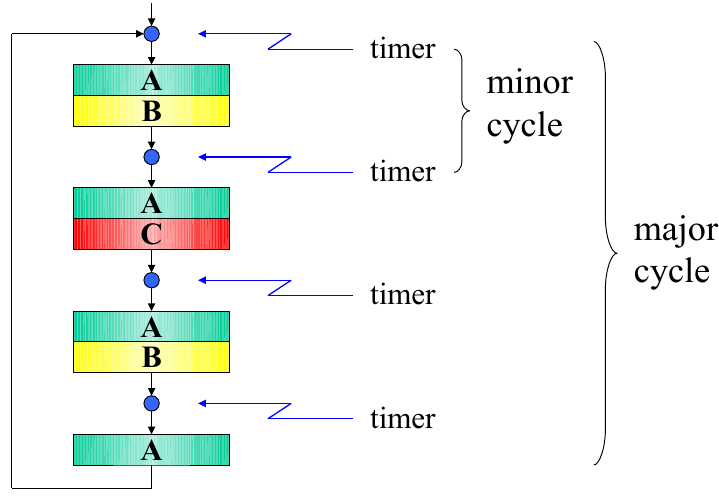
\includegraphics[width=0.5\textwidth]{img/ts}
\end{figure}
\begin{tabular}{ p{7.25cm} | p{7.25cm} }
    \textcolor{green}{\textbf{Vantaggi}} & \textcolor{red}{\textbf{Svantaggi}} \\
    \textbf{-} implementazione semplice (non viene richiesto alcun sistema operativo \textit{real-time}) &  \textbf{-} non è robusto contro \textit{overload} del sistema \\
    \textbf{-} ogni procedura condivide un \textit{address space} comune & \textbf{-} nel caso di aggiunta di un nuovo task è molto difficile l'espansione dello \textit{scheduler} \\
    \textbf{-} basso \textit{overhead} a tempo di esecuzione & \textbf{-} non è facile gestire task aperiodici \\
    \textbf{-} permette di controllare i \textit{jitter} & \textbf{-} tutti i processi devono avere periodo multiplo del \textit{minor cycle} \\
     & \textbf{-} è difficile includere processi con un periodo lungo \\
     & \textbf{-} difficile da costruire e da mantenere \\
     & \textbf{-} tutti i processi con un \textit{WCET} variabile devono essere \textit{splittati} in procedure con lunghezza fissa. (il determinismo non è richiesto, ma la predicibilità si) \\
\end{tabular}
\\ \newline
Durante un \textbf{\textit{overload}} si possono ``considerare'' due vie: la prima è quella di lasciar finire il task, che però comporta un \textbf{effetto domino} che va a portare delle ripercussioni anche su tutti gli altri task e che potrebbe portare ad un \textbf{\textit{timeline break}}; il secondo caso è gestire l'\textit{overload} con l'interruzione del task, in questo caso il sistema potrebbe rimanere in uno stato \textbf{inconsistente}. In un altro caso si ha necessità di incrementare il \textit{WCET} di un task, ma se al somma dei \textit{WCET} dei task in esecuzione nel $\Delta$ è maggiore del $\Delta$, allora sarà necessario dividere uno degli $n$ task in quel $\Delta$ di tempo in modo da evitare un \textit{timeline break}.
\begin{center}
    \begin{tabular}{ | c | c | c | } \hline
        \textbf{task} & $T$ & $T'$ \\ \hline
        $A$ & 25 ms & 25 ms \\ \hline
        $B$ & 50 ms & 40 ms \\ \hline
        $C$ & 100 ms & 100 ms \\ \hline
        \textbf{\textit{minor cycle}} & $\Delta$ = 25ms & $\Delta$ = 5ms \\ \hline
        \textbf{\textit{major cycle}} & $\mathbf{T}$ = 100ms & $\mathbf{T}$ = 200ms \\ \hline
    \end{tabular}
\end{center}

\section{Priority Scheduling}
Ad ogni task viene assegnata una priorità basata sui sui vincoli temporali, è possibile verificare la fattibilità di uno \textit{schedule} usando tecniche analitiche. I task sono eseguiti su un \textit{priority-based kernel}.

\subsection{Rate Monotonic}
Ad ogni task viene assegnata una \textbf{priorità fissa} in maniera proporzionale alla sua frequenza. In caso di \textit{overhead} sull'esecuzioni di singoli job l'\textbf{RM} è più solido del \textit{timeline schedule}.
\begin{figure}[h]
    \centering
    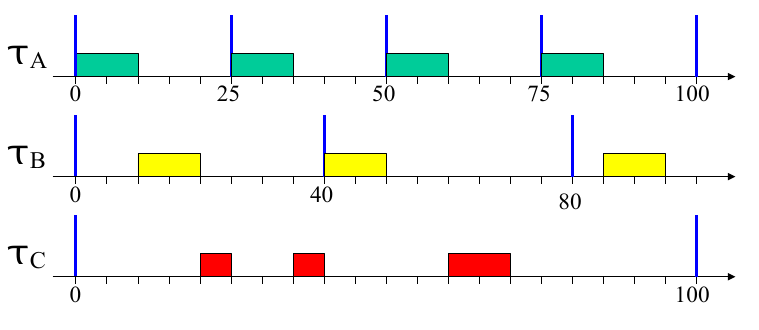
\includegraphics[width=0.5\textwidth]{img/rm_1}
\end{figure}
\\
Definiamo l'utilizzazione della \textit{CPU} da parte di un task come $U_i = \frac{C_i}{T_i}$, in questo modo possiamo andare a calcolare l'utilizzazione della \textit{CPU} su tutti i task definiti:
\begin{center}
    \[U_p = \sum_{i = 1}^{n} \frac{C_i}{T_i} \qquad \leftarrow U_p \text{ processor load} \]
\end{center}
In questo modo riusciamo a valutare il \textbf{carico del processore} che però \textbf{non} è una condizione \textbf{sufficiente} per garantire la \textbf{\textit{schedulabilità}} di un \textit{task set}, ma solo \textbf{necessaria}, infatti ci può dire se il \textit{task set} non è schedulabile in quanto $U_p > 1$ indica che il processore è \textit{overloaded}, ma nel caso in cui $U_p < 1$ ci possono essere dei casi in cui il \textit{task set} non può essere schedulato tramite \textit{RM}. \\
È possibile però identificare un punto, noto come $U_{lub}$ [\textit{least upper bound}] tale per cui sia possibile avere un \textbf{test di schedulabilità} sia \textbf{necessario} che \textbf{sufficiente}. Infatti nel caso in cui $U_p \leq U_{lub}$ il \textit{task set} è sicuramente schedulabile tramite \textit{RM}. Mentre nel caso in cui $U_{lub} < U_p \leq 1$ non possiamo dire niente di certo sulla fattibilità del \textit{task set}.
Per \textit{Rate Monotonic} $U_p^{RM} = n \cdot (2^{\frac{1}{n}} - 1)$ quindi avremo che: \[ \lim_{n\to\infty} U_{lub} = \log_2 2\]
Definiamo il \textbf{\textit{Critical Instant}} come l'istante di tempo in cui è presente il \textit{response time} maggiore, è stato dimostrato che equivale, considernado un \textit{task set} $\mathcal{T}$ all'istante in cui arrivano in corrispondenza tutti i task a più alta priorità. \\
Dal punto di vista della schedulabilità un task sporadico può essere considerato come un task periodico e quindi è possibile calcolarsi il suo $U_p$ e confrontarlo con l'$U_{lub}$ del \textit{task set}. \\
\textbf{\textit{Rate Monotonic}} è \textbf{ottimo}, infatti se esiste un assegnamento a priorità fisse che permette la fattibilità di uno \textit{schedule} per un \textit{task set} $\mathcal{T}$ allora l'assegnamento \textit{RM} è fattibile per il \textit{task set} $\mathcal{T}$, al contrario se un \textit{task set} non è schedulabile con \textit{RM} allora non esiste nessun altro assegnamento a priorità fissa che riesca a rendere fattibile la schedulazione del \textit{task set}. \\
\textbf{\textit{Hyperbolic Bound}}: \[ \prod_{i=1}^n (U_i + 1) \leq 2 \qquad \text{vs.} \qquad \sum_{i=1}^n U_i \leq n \cdot (2^{\frac{1}{n}} - 1)\]

\section{Earliest Deafline First}
Ogni \textit{job} riceve una \textit{deadline \textbf{assoluta}} $d_{i,k} = r_{i,k} + D_i$, in ogni istante di tempo il processore viene assegnato al \textit{job} con la \textit{earliest absolute deadline}, con EDF, qualsiasi set di attività può utilizzare il processore fino al 100\%. \\
\textbf{EDF} è \textbf{ottimale} ovvero se esiste uno \textit{schedule} per $\mathcal{T}$ allora \textbf{EDF} genererà uno \textit{schedule} fattibile, viceverse se $\mathcal{T}$ non è schedulabile con \textbf{EDF} allora non sarà schedulabile per nessun altro algoritmo di scheduling.
Nel caso di \textbf{EDF} il test \textbf{necessario} e \textbf{sufficiente} affinché un \textit{task set} sia schedulabile è che $U_p \leq 1$.
\begin{center}
    \begin{tabular}{ c | c } 
        \textbf{EDF} & \textbf{RM} \\
        \textbf{-} è molto più efficente & \textbf{-} è più semplice implementarla su un sistema operativo commerciale \\ 
        \textbf{-} riduce i \textit{context switches} & \textbf{-} è più predicibile durante \textit{overload} \\
    \end{tabular}
\end{center}

\newpage
\section{Task $D_i \leq T_i$}
Andiamo ora a considerare il caso in cui un task $\tau_i(C_i, D_i, T_i)$ ovvero in cui la \textit{deadline} assoluta non coincide con il \textit{request time} ovvero in cui $D_i < T_i$. In questi casi possiamo utilizzare due tipologie diverse di \textit{scheduler}:
\begin{itemize}
    \item \textbf{\textit{fixed priority}}: \textbf{\textit{Deadline Monotonic}} $p_i \propto \frac{1}{D_i}$
    \item \textbf{\textit{dynamic priority}}: \textbf{\textit{Earliest Deadline First}} $p_i \propto \frac{1}{d_i}$
\end{itemize}
\begin{figure}[h]
    \centering
    \begin{minipage}[t]{0.45\textwidth}
        \centering
        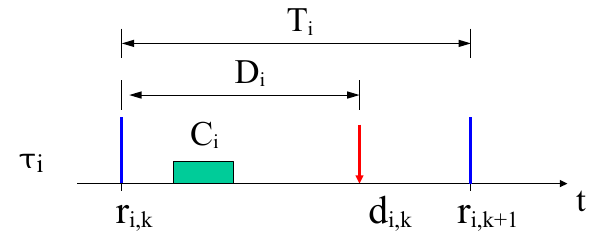
\includegraphics[width=\textwidth]{img/d_less_t_task}
        \caption{\textit{task} con $D_i \leq T_i$}
    \end{minipage}
    \begin{minipage}[t]{0.45\textwidth}
        \centering
        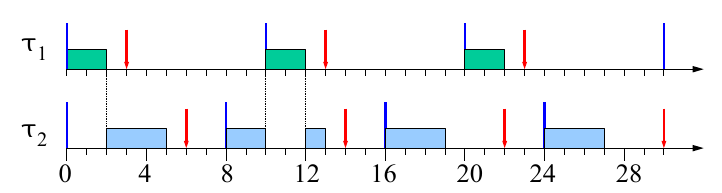
\includegraphics[width=\textwidth]{img/dm_1}
        \caption{\textit{deadline monotonic}}
    \end{minipage}
\end{figure}

\section{Response Time Analysis}
Siccome nel caso di uno scheduler \textit{deadline monotonic} ricavare l'\textit{utilization bound} non è utile in quanto sono fattibili anche \textit{task set} con $U_p > 1$. \\
Il \textit{response time analysis} è un test \textbf{sufficiente} e \textbf{necessario} per la schedulabilità di un \textit{task set} $\tau_i$, per ogni task $\tau_i$ calcolare l'\textit{iterference} $I_i$ che può essere causata da task a più alta priorità, possiamo quindi ora calcolare il \textit{response time} come $R_i = C_i + I_i$ e possiamo verificare che questo sia minore della \textit{deadline} relativa $R_i \leq D_i$. \\
Per calcolare l'interferenza di un task $\tau_k$ (a priorità alta) su $\tau_i$ (a priorità minore) nell'intervallo $[0, R_i]$: \[ I_{ik} \lceil \frac{R_i}{T_k} \rceil \cdot C_k \rightarrow I_k = \sum_{k=1}^{i-1} \lceil \frac{R_i}{T_k} \rceil \cdot C_K \]
Il calcolo del \textbf{\textit{response time}} è invece iterativo:
\begin{center}
    \begin{math}
        \begin{cases}
            R_i^0 = C_i \\
            R_i^{(s+1)} = C_i + \sum_{k=1}^{i-1} \cdot \lceil \frac{R_i^{(s)}}{T_k} \rceil \cdot C_k
        \end{cases}
        \rightarrow R_i^{(s+1)} = R_i^{(s)}
    \end{math}
\end{center}
\newpage
\textcolor{yellow}{\textbf{Esercizio}} \\
Consideriamo un \textit{task set} del tipo:
\begin{math}
    \begin{cases}
        \tau_1 = (3, 6) \\
        \tau_2 = (7, 28) \\
        \tau_3 = (5, 28, 30)
    \end{cases}
\end{math} \\ \newline
andiamo prima a valutare la \textit{schedulabilità} andando a calcolare l'\textit{utiliation bound} modificata (quindi con le \textit{deadline} e non con i periodi), visto che c'è almeno un task che ha $T_i \neq D_i$.
\begin{center}
    \begin{math}
        \begin{aligned}
            U_p^* &= \frac{C_1}{D_2} + \frac{C_2}{D_2} + \frac{C_3}{D_3} \\
            &= \frac{3}{6} + \frac{7}{28} + \frac{5}{28} = 0.93 \qquad \stackrel{\text{?}}{\leq} \qquad U_p^* = n \cdot (\sqrt[n]2 - 1) = 0.78\\
        \end{aligned}
    \end{math}
\end{center}
\begin{itemize}
    \item $\tau_1 \rightarrow R_i = C_i - I_i = 3 - 0 = 3 \stackrel{\text{?}}{\leq} 6$ \textbf{OK}. \\
    Il task $\tau_1$ è \textbf{schedulabile}, siccome siamo in priorità fisse.
    \item il task $\tau_2$ è \textbf{schedulabile}
    \begin{center}
        $R_2 = C_2 + \lceil \frac{R_2}{T_1} \rceil \cdot C_1 = 7 + \lceil \frac{7}{6} \rceil \cdot 3 = 13 \stackrel{\text{?}}{=} 7 \; \mathbf{NO}$ \\
        $R'_2 = 7 + \lceil \frac{13}{6} \rceil \cdot 3 = 16 \stackrel{\text{?}}{=} 13 \; \mathbf{NO}$ \\
        $R''_2 = 7 + \lceil \frac{16}{6} \rceil \cdot 3 = 16 \stackrel{\text{?}}{=} 16 \; \mathbf{SI} \stackrel{\text{?}}{\leq} 28 \; \mathbf{OK}$ 
    \end{center}
    \item il task $\tau_3$ è \textbf{schedulabile}
    \begin{center}
        \begin{math}
            \begin{aligned}
                R_3 &= C_3 +  \lceil \frac{R_3}{T_1} \rceil \cdot C_1  + \lceil \frac{R_3}{T_2} \rceil \cdot C_2 \\
                &= 5 +  \lceil \frac{5}{6} \rceil \cdot 3  + \lceil \frac{5}{28} \rceil \cdot 7 = 15 \stackrel{\text{?}}{=} 5 \; \mathbf{NO} \\
                R'_3 &= 5 +  \lceil \frac{15}{6} \rceil \cdot 3  + \lceil \frac{15}{28} \rceil \cdot 7 = 21 \stackrel{\text{?}}{=} 15 \; \mathbf{NO} \\
                R''_3 &= 5 +  \lceil \frac{21}{6} \rceil \cdot 3  + \lceil \frac{21}{28} \rceil \cdot 7 = 24 \stackrel{\text{?}}{=} 21 \; \mathbf{NO} \\
                R''_3 &= 5 +  \lceil \frac{24}{6} \rceil \cdot 3  + \lceil \frac{24}{28} \rceil \cdot 7 = 24 \stackrel{\text{?}}{=} 24 \; \mathbf{SI} \stackrel{\text{?}}{\leq} 28 \; \mathbf{OK}\\
            \end{aligned}
        \end{math}
    \end{center}
\end{itemize}
Possiamo quindi affermare che l'intero \textit{task set} $\mathcal{T}$ è \textbf{schedulabile}, ed ha una complessità pari a: $\mathcal{O}(n \cdot D_{max})$.
\newpage
\section{Processor Demand Criterion}
In ogni intervallo di tempo la \textit{computation demanded} dal \textit{task set} non deve essere maggiare del tempo disponbiie. Nel caso di \textbf{EDF} abbiamo priorità dinamiche ed è quindi impossibile utilizzare il \textit{response time analysis} per dire se un \textit{task set} è schedulabile. \\
La \textbf{\textit{demand}} in $[t_1, t_2]$ è il \textit{WCET} di quei task che anno $r_i \geq t_1 \cap d_i \leq t_2$: \[ g(t_1, t_2) = \sum_{r_i \geq t_1}^{d_i \leq t_2} C_i\]
Consideriamo ora $t_1 = 0$ (ovvero il \textit{critical istance}) e $t_2 = \mathcal{L}$ e andiamo a calcolarci la \textbf{\textit{demand}} nell'intervallo di tempo $[0, \mathcal{L}]$ allora avremo che: \[g(0, \mathcal{L}) = \sum_{r_i \geq 0}^{d_i \leq \mathcal{L}} C_i = \sum_{i=1}^n \underbrace{\lfloor \frac{\mathcal{L} - D_i + T_i}{T_i} \rfloor}_{\text{Quando i task hanno }r_i\text{ e }d_i \text{ all'interno di }\mathcal{L}} \cdot C_i\]
L'\textit{execution time demanded} dai singoli \textit{job} che hanno \textit{deadline} $d_i \leq \mathcal{L}$ su un intervallo di lunghezza $\mathcal{L}$ non può essere maggiore di $\mathcal{L}$ ovvero \[ \forall \mathcal{L} > 0 \; g(0, \mathcal{L}) \leq \mathcal{L} \qquad \leftarrow \text{è inapplicabile } \mathcal{L} \rightarrow \infty \]
\begin{figure}[h]
    \centering
    \begin{minipage}[t]{0.45\textwidth}
        \centering
        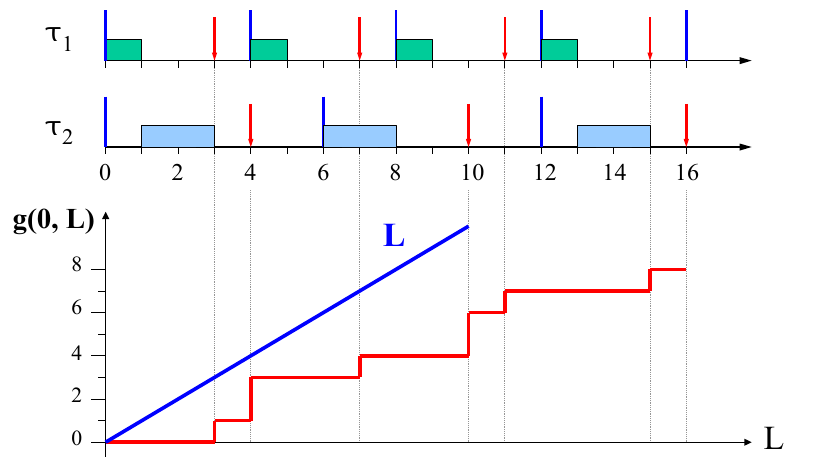
\includegraphics[width=\textwidth]{img/pdc_1}
    \end{minipage}
    \begin{minipage}[t]{0.45\textwidth}
        \centering
        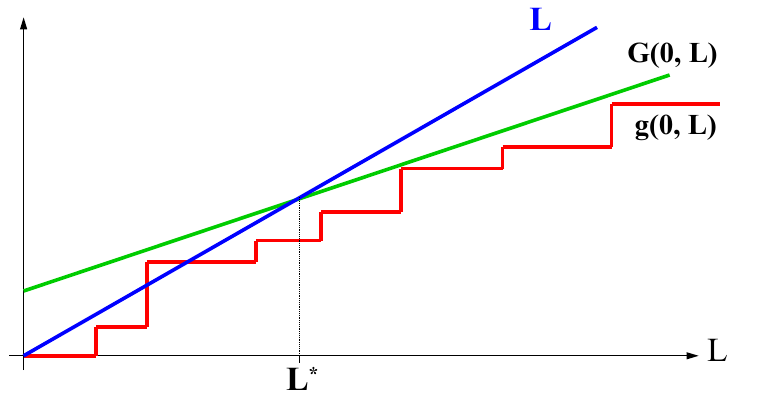
\includegraphics[width=\textwidth]{img/pdc_2}
    \end{minipage}
\end{figure}
\\
Controllare la schedulabilità utilizzando la funzione $g(0, \mathcal{L})$ che è continua nell'intervallo $[0, \mathcal{L}]$ \textbf{non} è \textbf{fattibile}. Possiamo però rendere la funzione un \textit{staircase function} con dei salti (discontinuità) nei punti di \textit{deadline} assoluta $d_{i,k} = (k - 1) \cdot T_i + D_i$, perché possiamo notare dalla figura che i punti in cui la \textit{demand} rischia di superare $\mathcal{L}$ sono nei punti di \textbf{discontinuità}. Possiamo identificare un \textbf{\textit{hyberperiod} H} dopo il quale il comportamento della nostra funzione discontinua si ripeterà, $\mathbf{H} = lcm(T_i, T_j) \; \forall T_i,T_j \in \mathcal{T} \; con \; i \neq j$ ovvero il minimo comune multiplo tra i periodi del \textit{task set}. \\
\[g(0, \mathcal{L}) = \sum_{i=1}^n \lfloor \frac{\mathcal{L} + T_i - D_i}{T_i} \rfloor \cdot C_i\]
\[G(0, \mathcal{L}) = \sum_{i=1}^n (\frac{\mathcal{L} + T_i - D_i}{T_i})  \cdot C_i\]
Per definizione del \textit{floor} avremo che $g(0, \mathcal{L}) \leq G(0, \mathcal{L})$.
\begin{equation}
    \begin{alignedat}{2}
        G(0, \mathcal{L}) &= \sum_{i=1}^n (\frac{\mathcal{L} + T_i - D_i}{T_i}) \cdot C_i \\
        &= \sum_{i=1}^n \frac{\mathcal{L}}{T_i} \cdot C_i + (\frac{T_i - D_i}{T_i}) \cdot C_i \\
        &= \sum_{i=1}^n \mathcal{L} \cdot \underbrace{\frac{C_i}{T_i}}_{U} + (T_i - D_i) \cdot \underbrace{\frac{C_i}{T_i}}_{U_i} \\
        &= \mathcal{L}U \cdot \sum_{i=1}^n (T_i - D_i) \cdot U_i
    \end{alignedat}
\end{equation}
Ora vogliamo trovare il punto di intersezione $\mathcal{L}^*$ tra $\mathcal{L}$ e $G(0, \mathcal{L})$, poniamo quindi: 
\begin{equation}
    \begin{alignedat}{2}
        \mathcal{L} &= G(0, \mathcal{L}) \\
        \mathcal{L} &= \mathcal{L}U \cdot \sum_{i=1}^n (T_i - D_i) \cdot U_i \\
        \mathcal{L} - \mathcal{L}U &= \sum_{i=1}^n (T_i - D_i) \cdot U_i \\
        \mathcal{L} \cdot (1 - U) &= \sum_{i=1}^n (T_i - D_i) \cdot U_i \\
        \mathcal{L}^* &= \frac{\sum_{i=1}^n (T_i - D_i) \cdot U_i}{1 - U}
    \end{alignedat}
\end{equation}
Per verificare quindi se il \textit{task set} è schedulabile dovremo valutare se $\forall \mathcal{L} \in D, \; g(0, \mathcal{L}) \leq \mathcal{L}$ dove avremo che:
\begin{center}
    \begin{math}
        D = \{d_k | d_k \leq \min (\mathbf{H}, \mathcal{L}^*)\}
        \begin{cases}
            \mathbf{H} = lcm(T_i, T_j) \; \forall T_i,T_j \in \mathcal{T}, \; i \neq j \\
            \mathcal{L}^* = \frac{\sum_{i=1}^n (T_i - D_i) \cdot U_i}{1 - U}
        \end{cases}
    \end{math}
\end{center}
\newpage
\textcolor{yellow}{\textbf{Esercizio}} \\
Consideriamo il seguente \textit{task set}: 
\begin{math}
    \begin{cases}
        \tau_1(1, 2, 3) \\
        \tau_2(2, 5.5, 7) \\
        \tau_3(2, 6, 10)
    \end{cases}
\end{math}
\\ \newline
Identifichiamo come prima cosa la nostra $D$: 
\begin{center}
    \begin{math}
        D = \{d_k | d_k \leq \min (\mathbf{H}, \mathcal{L}^*)\}
        \begin{cases}
            \mathbf{H} = lcm(T_1, T_2, T_3) = lcm(3, 7, 10) = 210 \\
            \begin{aligned}
                \mathcal{L}^* &= \frac{\sum_{i=1}^n (T_i - D_i) \cdot U_i}{1 - U} \\ 
                &= \frac{[(3 - 2) \cdot \frac{1}{3}] + [(7 - 5.5) \cdot \frac{2}{7}] + [(10 - 6) \cdot \frac{2}{10}]}{1 - \underbrace{(\frac{1}{3} + \frac{2}{7} + \frac{2}{10})}_{U_{lub} \; = \; 0.8190}} \\
                &= 8.63
            \end{aligned}
        \end{cases}
    \end{math}
\end{center}
\begin{itemize}
    
    \item consideriamo $\mathcal{L} = 2$
    \begin{center}
        $\lfloor \frac{\mathcal{L} + T_1 - D_1}{T_1} \rfloor \cdot C_1 = \lfloor \frac{2 + 3 - 2}{3} \rfloor \cdot 1 = 1 \stackrel{\text{?}}{\leq} 2 \qquad \leftarrow $ \textbf{OK}
    \end{center}
    \item consideriamo $\mathcal{L} = 5$
    \item consideriamo $\mathcal{L} = 5.5$
    \begin{center}
        \begin{math}
            \begin{aligned}
                g(0, \mathcal{L}) &= \lfloor \frac{\mathcal{L} + T_1 - D_1}{T_1} \rfloor \cdot C_1 + \lfloor \frac{\mathcal{L} + T_2 - D_2}{T_2} \rfloor \cdot C_2 \\
                &= \lfloor \frac{5.5 + 3 - 2}{3} \rfloor \cdot 1 + \lfloor \frac{5.5 + 7 - 5.5}{7} \rfloor \cdot 2 \\
                &= 2 + 2 = 4 \stackrel{\text{?}}{\leq} 5.5 \qquad \leftarrow \; \mathbf{OK}
            \end{aligned}
        \end{math}
    \end{center}
    \item consideriamo $\mathcal{L} = 6$
    \begin{center}
        \begin{math}
            \begin{aligned}
                g(0, \mathcal{L}) &= \lfloor \frac{\mathcal{L} + T_1 - D_1}{T_1} \rfloor \cdot C_1 + \lfloor \frac{\mathcal{L} + T_2 - D_2}{T_2} \rfloor \cdot C_2 + \lfloor \frac{\mathcal{L} + T_3 - D_3}{T_3} \rfloor \cdot C_3 \\
                &= \lfloor \frac{6 + 3 - 2}{3} \rfloor \cdot 1 + \lfloor \frac{6 + 7 - 5.5}{7} \rfloor \cdot 2 + \lfloor \frac{6 + 10 - 6}{10} \rfloor \cdot 2 \\
                &= 2 + 2 + 2 = 6 \stackrel{\text{?}}{\leq} 6 \qquad \leftarrow \; \mathbf{OK}
            \end{aligned}
        \end{math}
    \end{center}
    \item consideriamo $\mathcal{L} = 8$
    \begin{center}
        \begin{math}
            \begin{aligned}
                g(0, \mathcal{L}) &= \lfloor \frac{\mathcal{L} + T_1 - D_1}{T_1} \rfloor \cdot C_1 + \lfloor \frac{\mathcal{L} + T_2 - D_2}{T_2} \rfloor \cdot C_2 + \lfloor \frac{\mathcal{L} + T_3 - D_3}{T_3} \rfloor \cdot C_3 \\
                &= \lfloor \frac{8 + 3 - 2}{3} \rfloor \cdot 1 + \lfloor \frac{8 + 7 - 5.5}{7} \rfloor \cdot 2 + \lfloor \frac{8 + 10 - 6}{10} \rfloor \cdot 2 \\
                &= 3 + 2 + 2 = 7 \stackrel{\text{?}}{\leq} 8 \qquad \leftarrow \; \mathbf{OK}
            \end{aligned}
        \end{math}
    \end{center}
\end{itemize}

\resizebox{\textwidth}{!}{%
\begin{forest}
  for tree={
    child anchor=west,
    parent anchor=east,
    grow'=east,
    text width=4cm,
    draw,
    anchor=west,
    edge path={
      \noexpand\path[\forestoption{edge}]
        (.child anchor) -| +(-5pt,0) -- +(-5pt,0) |-
        (!u.parent anchor)\forestoption{edge label};
    },
  }
    [\textbf{Periodic Tasks}
        [\textit{deadline} uguali al periodo: $D_i \stackrel{\text{?}}{=} T_i$
            [\textbf{\textit{Rate Monotonic}}
                [ \textit{optimaily}]
                [ \textit{bounds}
                    [\textit{classical}]
                    [\textit{hyperbolic}]
                ]
            ]
            [ \textbf{\textit{Earliest Deadline First}}
                [\textit{bounds}]
                [\textit{optimaility}]
            ]
        ]
        [\textit{deadline} minore del periodo: $D_i \stackrel{\text{?}}{\leq} T_i$
            [ \textbf{\textit{Deadline Monotonic}}
                [ \textit{per task tests}
                    [\textit{simple}]
                    [\textit{recursive}]
                    [\textit{response time analysis}]
                ]
                [\textit{bounds}]
            ]
            [ \textbf{\textit{Earliest Deadline First}}
                [\textit{processor demand criterion}]
            ]
        ]
    ]
\end{forest}
}


\resizebox{\textwidth}{!}{%
\begin{forest}
  for tree={
    child anchor=west,
    parent anchor=east,
    grow'=east,
    text width=4cm,
    draw,
    anchor=west,
    edge path={
      \noexpand\path[\forestoption{edge}]
        (.child anchor) -| +(-5pt,0) -- +(-5pt,0) |-
        (!u.parent anchor)\forestoption{edge label};
    },
  }
    [ \textbf{RIASSUNTONE}
        [\textbf{Scheduling Approaches}
            [ costruzione offline
                [\textbf{\textit{timeline scheduling}}]
            ]
            [ priorità \textbf{fisse}
                [\textbf{\textit{rate monotonic}}]            
                [\textbf{\textit{deadline monotonic}}]
            ]
            [ priorità \textbf{dinamiche}
                [\textbf{\textit{Earliest Deadline First}}]
            ]
        ]
        [ \textbf{Analysis Techniques}
            [ \textbf{\textit{Processor Utilization Bound}}
                [test \textbf{sufficente}]
                [$U \leq U_{lub}$
                    [$\mathcal{O}(n)$]
                ]
            ]
            [ \textbf{\textit{Response Time Analysis}}
                [test sia \textbf{sufficente} che \textbf{necessario} per \textit{RM} e \textit{DM}]
                [$\forall i \; R_i \leq D_i$
                    [$\mathcal{O}(n \cdot D_{max})$]
                ]
            ]
            [ \textbf{\textit{Processor Demand Criterion}}
                [test sia \textbf{sufficente} che \textbf{necessario} per \textit{EDF}]
                [$\forall \mathcal{L} \; g(0; \mathcal{L}) \leq \mathcal{L}$
                    [\textit{psuedo-polynomial} $U \stackrel{\text{?}}{<}1$]
                ]
            ]
        ]
    ]
\end{forest}
}



% PAGINA VUOTA
%\clearpage\null\thispagestyle{empty}\clearpage
%\appendix
%\appendixpage
%\addappheadtotoc

%\clearpage\null\thispagestyle{empty}\clearpage


%\listoffigures


\begin{flushleft}
\bibliographystyle{plain}
\bibliography{sections/references} 
\end{flushleft}

\end{document}
